\section{Grundlagen}
\label{sec:Grundlagen}

Zum besseren Verständnis der Arbeit werden hier die wichtigsten Begriffe definiert, Gründe dieser Arbeit werden erläutert und die Vorgehensmethoden des Reviews erklärt.

\subsection{Definition}
\label{subsec:Definition}

\begin{description}
	\item [Codereview:]
		Unter Codereview versteht man, eine manuelle Überprüfung des Quellcodes durch andere Entwickler als den Autor. Es gilt als wertvolles Werkzeug zur Reduzierung von 							Softwarefehlern und zur Verbesserung der Qualität von Softwareprojekten \cite{bacchelli2013expectations}.

	\item [\ac{VCS}:]
		"`Versionskontrollsysteme sind Softwaretools, mit deren Hilfe Softwareteams Quellcodeänderungen verwalten können. Die Versionskontrollsoftware verfolgt jede Änderung am Code und 		speichert sie in einer speziell hierfür angelegten Datenbank. Unterläuft einem Entwickler ein Fehler, kann er einen Schritt zurück machen, seinen Code mit früheren Codeversionen 		abgleichen und Korrekturen implementieren. Und das mit minimalen Beeinträchtigungen für seine Teamkollegen."' \cite{version-control-System}
		
		Beispiele dafür sind:
		\begin{itemize}
			\item Git: Ist eine freie und Open-Source Software zur Versionsverwaltung von Dateien, das 2005 ursprünglich von Linus Torvalds, dem berühmten Entwickler des Linux 						Betriebssystem-Kernel, entwickelt wurde.
			\item SVN: Apache Subversion ist eine freie Software zur zentralen Versionsverwaltung von Dateien und Verzeichnissen. Die Versionierung erfolgt in einem zentralen Repository 			in Form einer Revisionszählung.
		\end{itemize}
	
	\item[Commit:] Ist ein Ausdrück, der eine dokumentierte Änderung einer Datei im \ac{VCS} beschreibt. Jedes Commit ist bekannt durch ein bestimmtes ID.
	Für das Review ist es wichtig zu unterscheiden zwischen den folgenden zwei commits Methoden:
	
	\begin{itemize}	
	\item \textbf{Post-commit:}
		Die Überprüfung erfolgt, nachdem die Änderungen am Quelltext an das Ziel-Repository gesendet wurde.
		\begin{description}
			\item [Vorteile:] \hfill
			\begin{enumerate}
				\item Andere Teammitglieder sehen die Codeänderungen und können ihre Arbeit entsprechend ändern
				\item Dieser Prozess kann praktisch sein, weil einige Änderungen komplex und lang sein können und mehrere Schritte für den Review erfordern
			\end{enumerate}
			
			\item[Nachteile:] \hfill
			\begin{enumerate}
				\item Erhöhte Wahrscheinlichkeit, dass schlechter Code in das Haupt Repository gelangt, was sich auf die Arbeit des gesamten Teams auswirkt
				\item Wenn Fehler gefunden werden, kann es eine Weile dauern, bis der Entwickler zu dem Modul zurückkehrt, an dem er gearbeitet hat
			\end{enumerate}
		\end{description}
		
	\item \textbf{pre-commit:}
		Ist eine Art des Reviews, mit der man die Änderungen des Quelltextes überprüft, bevor die in das Haupt-Repository des Versionsverwaltungssystems gelangen.
		\begin{description}
		
			\item [Vorteile:] \hfill
			\begin{enumerate}
				\item Diese Art erstellt eine Art von Sicherheit, da fehlerhafte oder unvollständige Änderungen durch den Review auftreten können
				\item Dieser Prozess stellt sicher, dass der Autor seine Änderungen überprüfen lässt und nicht direkt in das Ziel-Repository eincheckt
			\end{enumerate}
		
			\item [Nachteile:] \hfill
			\begin{enumerate}
				\item Es besteht keine Möglichkeit mehr, um bestehende Commits zu überprüfen
				\item Kostet viel Zeit, da durch Verwendung dieser Methode muss jede Änderung unabhängig von der Größe zuerst angeschaut werden
			\end{enumerate}
			
		\end{description}	
	\end{itemize}
				
	\item [Pull Request:]
		Ist eine Anfrage, die die neue Features enthält und an die Reviewer abschickt wird, um Änderungen am Code zu überprüfen. Meistens arbeiten die Entwickler an einem abgespaltenen 			Zweig vom Ziel branch und sobald er fertig ist, sendet er die Anfrage zur Überprüfung an die Reviewer. Wird ein Pull-Request angenommen, werden die Änderungen mit dem Ziel- 				Branch zusammengeführt. wird das Pull Request abgelehnt, werden die Änderungen bearbeitet und wird eine neue Anfrage benötigt.
	
	\item [Continuous Integration (CI):]
		"`CI bedeutet Continuous Integration, also der Automatisierungsprozess für Entwickler. Bei einer erfolgreichen CI werden regelmäßig neue Codeänderungen für Apps entwickelt, 				geprüft und in einem gemeinsamen Repository zusammengeführt. Damit soll der Konflikt verhindert werden, den zu viele Branches einer App verursachen können, wenn sie zeitgleich 			entwickelt werden."' \cite{RedHat}
			
	\item [Continuous Delivery (CD):]
		"`Continuous Delivery bedeutet üblicherweise, dass App Änderungen eines Entwicklers automatisch auf Bugs getestet und in ein Repository (wie GitHub oder eine Container 					Registry) hochgeladen werden, von wo aus sie vom Operations-Team in einer Live-Produktivumgebung bereitgestellt werden können. Dieser Vorgang ist die Antwort auf Transparenz- 				und Kommunikationsprobleme zwischen Dev- und Business-Teams. Damit soll sichergestellt werden, dass neuer Code mit minimalem Aufwand implementiert werden kann."' \cite{RedHat}
		
	\item [Continuous Deployment (CD):]
		"`Continuous Deployment (das andere „CD“) kann sich auf die automatische Freigabe von Entwickleränderungen vom Repository zur Produktivphase beziehen, wo sie direkt vom Kunden 			genutzt werden können. Dieser Vorgang soll der Überlastung von Operations-Teams bei manuellen Prozessen entgegenwirken, die die Anwendungsbereitstellung verlangsamen. Continuous 		Development baut die Vorteile der Continuous Delivery aus, indem auch noch die nächste Phase der Pipeline automatisiert wird."' \cite{RedHat}

	Dieser Prozess kann als eine Pipeline vorgestellt werden, die die \cref{fig:RedHat} beschreibt.
	\begin{figure}[H]
		\centering
		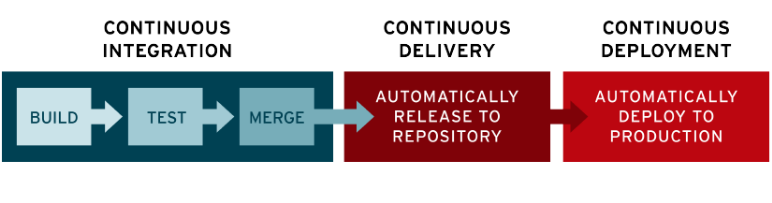
\includegraphics[width=1.0\textwidth]{Red Hat CI CD}
		\caption[\ac{CI}/\ac{CD}]{\ac{CI}/\ac{CD} Prozess als Pipeline\\ \cite{RedHat}}
		\label{fig:RedHat}
	\end{figure}
	
\end{description}

\subsection{Motivation}
\label{subsec:Gründe}
Durch den Review des Codes entstehen zahlreiche Vorteile. Zum Beispiel:

\begin{enumerate}
	\item Frühzeitige Erkennung von Fehlern im Quellcode, denn es ist immer umständlich, wenn erst nach einer Weile einen Fehler auftritt, was eine ältere Änderung verursachte.
		Fehler müssen nicht nur, diejenige die das Programm nicht mehr lauffähig machen, sondern können auch Falsche Schnittstellenspezifikation oder Verletzung von Namenskonventione 
		etc.\ sein.
	\item Fehler die erst beim Kunden auftreten, weil vorher keiner drüber geguckt hat kosten Geld und Reputation.
	\item Die Reviewer können durch lesen der Änderungen lernen.
	\item Der Autor kann durch Review-Kommentare lernen.
	\item Verbesserungsvorschläge und vielmehr.
\end{enumerate}

\subsection{Vorgehensmethoden}
\label{subsec:Vorgehensmethoden}
Es gibt verschiedene Verfahren von Reviews. Die am häufigsten benutzten Verfahren sind:
\unsure{Ändere den Artikel vom der zu das vom Wort Review in die ganze PA}
\begin{description}
	\item [Ad-hoc:] Der Review passiert nur für einen bestimmten Zweck und ist nicht zuvor geplant. Beispiel: Der Entwickler hat ein Feature entwickelt, so ruft er den Reviewer, der in 				der Regel mehr Erfahrungen hat, um die Änderungen zusammen zu diskutieren, bevor der Entwickler seine Änderungen eincheckt.
	\item [Over–the–shoulder:] Der Autor setzt direkt neben dem Reviewer, der die Änderungen kritisiert. Dieses Verfahren ist ein informeller Review.
	\item [Email pass-around:] Der Autor sendet eine E-Mail mit dem Code zur Überprüfung des Codes an die Reviewer.
	\item [Tool-assisted:] Hier werden Tools benutzt, die die Änderungen je nach Einstellung des Systems an die Rezensenten zum Überprüfen weiterleiten.
	\item [Reviewsitzung:] Das Team trefft sich regelmäßig, je nach Absprache. Diverse Meinungen werden dargestellt.
	\item [Stand Up Meeting:] Einmal am Tag werden die Änderungen diskutiert. Das Team muss nicht unbedingt dabei sein, sondern nur die für die Änderungen zuständig sind.
	\item [Planung:] Entwickler werden zur Review eingeladen, Rollen werden verteilt und die Ziele des Reviews werden festgelegt.
\end{description}

\textbf{Nachteile der Methoden die nicht Tool-basiert sind:}
\begin{itemize}
	\item Meistens werden zuerst die Änderungen im Quellcode geschrieben, was Fehler enthalten kann und danach kommt das Review.
	\item Dieser Prozess ist nicht flexibel, denn es fordert die Anwesenheit der für die Änderungen zuständige Personen zusammen mit den Rezensenten.
	\item Eine automatische Dokumentation des Reviews ist nicht möglich. D.h. wenn Benutzer das Review dokumentiert haben wollen, verlangt das eine manuelle Arbeit.
\end{itemize}

\subsection{Mögliche Git-Workflows}
\label{sec:Git-Workflows}

Git bietet die Möglichkeit, den Workflow an den Bedürfnisse des Teams anzupassen, daher gibt es unterschiedliche Workflows.

\begin{itemize}
	\item Feature-Branch-Workflow
	\item Git-flow-Workflow
\end{itemize}
werden hier vorgestellt.

\subsubsection{Feature-Branch-Workflow}
\label{subsubsec:Feature-Branch-Workflow}

Ziel dieses Workflows, dass ein anderer Branch statt dem Master-Branch (Haupt-Branch) für die Entwicklung von Features und die Review verwendet.
Ablauf: Vom Master-Branch wird einen Zweig erstellt, den der Entwickler zu seiner Arbeitskopie klont. So arbeitet er unabhängig von seinen Kollegen an einem bestimmten Feature und 		sobald er das Feature fertig hat, wird er seine Änderungen mit einem \code{push} in dem abgespaltenen Branch senden. Danach kann der Entwickler je nach Einstellungen des Systems den 	Review starten. Wird der Review z. B. mit einer Pull-Request gemacht werden, soll der Entwickler an dieser Stelle die Pull-Anfrage starten. So können sich die Reviewer die 				Änderungen anschauen, kommentieren und mit dem Autor diskutieren und am Ende diese Änderungen entweder annehmen oder ablehnen. Werden diese Änderungen angenommen, können direkt in 		das Master-Branch zusammengeführt werden \cite{Feature-Branch-Workflow}. Die \cref{fig:Forking-workflow} verdeutlicht diesen Prozess. 

\textbf{Eigenschaften dieses Verfahrens:}
\begin{itemize}
	\item Entwickler arbeiten nicht direkt an dem Haupt-Branch, demzufolge stören sie einander nicht
	\item Jedes Feature ist in einem Feature-Branch gekapselt
\end{itemize}

\subsubsection{Git-flow-Workflow}
\label{subsubsec:Git-flow-Workflow}

"`Der Git-flow-Workflow ist ein Git-Workflow, der von Vincent Driessen auf nvie veröffentlicht und bekannt gemacht wurde. Der Git-flow-Workflow definiert ein strenges Branching-Modell, das um den Release des Projekts konzipiert wurde. Dies bietet einen robusten Rahmen für das Management größerer Projekte.
Git-flow ist hervorragend für Projekte mit einem Release-Zyklus nach Zeitplan geeignet. Mit diesem Workflow werden keine neuen Konzepte oder Befehle hinzugefügt, die nicht auch für 		den Feature-Branch-Workflow erforderlich sind. Stattdessen werden verschiedenen Branches sehr spezifische Rollen zugewiesen, und es wird genau festgelegt, wann und wie die 				Interaktion erfolgen soll. Zusätzlich zu feature-Branches werden einzelne Branches zum Vorbereiten, Warten und Erfassen von Releases verwendet. Dabei kannst du natürlich auch alle 		Vorteile von Feature-Branch-Workflows nutzen: Pull-Anfragen, isolierte Tests und eine effizientere Zusammenarbeit."' \cite{Git-flow-Workflow}

Hier wird also ein anderer Branch (Develp-Branch) zusätzlich zum Master-Branch betrachtet. Dieses Branch wird für die Entwicklung verantwortlich sein, indem auf dem Master-Branch 			nur die Versionen zu sehen sind. Die Features werden in abgespaltenen Branchs vom Develop-Branch entwickelt und mit dem Develop-Branch nach einer erfolgreichem Pull-Anfrage 				zusammengeführt werden. Sind die Features auf dem develop-Branch soweit für eine neue Version, wird ein Release-Branch vom dvelop-Branch abgespalten, mit dem Release-Branch keine 			Features mehr von anderen Branchs zusammengeführt werden. Dieses Branch sagt einfach "`Ich bin die neue Version "'. Falls das Release-Branch Fehler enthält, kann die Behebung dieser			Fehler wieder in einem anderen Branch geschehen und in das Release-Branch zusammengeführt werden. Funktioniert die Version einwandfrei, wird sie mit dem Master-Branch 						zusammengeführt. Die \cref{fig:Git-flow-Workflow} soll bei der Vorstellung von diesem Workflow helfen.

\begin{figure}[H]
	\centering
	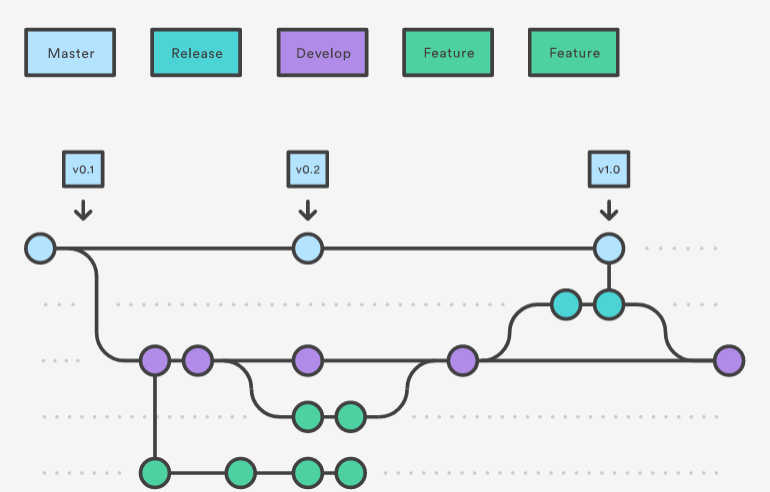
\includegraphics[width=0.9\textwidth]{Git-flow-Workflow}
	\caption[Git-flow-Workflow]{Git-flow-Workflow.\\ \cite{Git-flow-Workflow}}
	\label{fig:Git-flow-Workflow}
\end{figure}
	
\textbf{Eigenschaften dieses Verfahrens:}
\begin{itemize}
	\item Jedes Feature ist in einem Feature-Branch gekapselt
	\item Entwickler arbeiten nicht direkt an dem Haupt-Branch, demzufolge stören sie einander nicht
	\item Eignet sich gut für große Projekte, die mehrere Versionen enthalten sollen
	\item Dank des Develop-Branchs und der Release-Branchs hat das Master-Branch eine saubere Historie, da es auf dem Develop-Branchs statt dem Master-Branch entwickelt wird
\end{itemize}

